\documentclass{article} % For LaTeX2e
\usepackage{iclr2020_conference,times}
\usepackage{graphicx}
\usepackage{placeins}
\usepackage{flafter}
\usepackage{pgf-pie}
% Optional math commands from https://github.com/goodfeli/dlbook_notation.


\usepackage{hyperref}
\usepackage{url}


\title{Einfluss der Korpuszusammensetzung auf die Performance von audiobasierten Emotionserkennungssystemen}

% Authors must not appear in the submitted version. They should be hidden
% as long as the \iclrfinalcopy macro remains commented out below.
% Non-anonymous submissions will be rejected without review.

\author{Niels Lange \& Beate Zywietz\\
Institut für Maschinelle Sprachverarbeitung\\
Universität Stuttgart\\
Pfaffenwaldring 5, 70569 Stuttgart \\
\texttt{\{st158564, st155422\}@st.uni-stuttgart.de} \\
}
%The \author macro works with any number of authors. There are two commands
% used to separate the names and addresses of multiple authors: \And and \AND.
%
% Using \And between authors leaves it to \LaTeX{} to determine where to break
% the lines. Using \AND forces a linebreak at that point. So, if \LaTeX{}
% puts 3 of 4 authors names on the first line, and the last on the second
% line, try using \AND instead of \And before the third author name.

\newcommand{\fix}{\marginpar{FIX}}
\newcommand{\new}{\marginpar{NEW}}

\iclrfinalcopy % Uncomment for camera-ready version, but NOT for submission.
\begin{document}


\maketitle
\begin{abstract}

FORSCHUNGSFRAGE: "Welchen Einfluss hat die Zusammensetzung des verwendeten Korpus auf die Performance von DT und SVC?"
Wir haben beschlossen die classifier auf einem zweiten Korpus zu testen, als wir quasi nie über 45\% gekommen sind, um herauszufinden welche Schwierigkeiten auf die Qualität des verwendeten Korpus zurückzuführen sein könnten
\end{abstract}

\section{Einleitung und verwandte Literatur}

Emotionserkennung ist ein komplexe, anspruchsvolle Aufgabe. Auch uns Menschen gelingt es oft nicht, Gehörtes einstimmig einer Emotion zuzuordnen. 

Wie wir Stimuli interpretieren, ist hochgradig von unserem Wissen über den Gesprächskontext, unserem Verhältnis zu unserem Gesprächspartner und uns selbst als Person abhängig. Auch der kulturelle Hintergrund kann eine Rolle spielen. So wird zum Beispiel Russisch von Menschen, die selbst nicht Russisch sprechen, oft als aggressiv und übellaunig klingend beschrieben. 

Zudem gehen Emotionen in der Praxis fließend ineinander über. An welchem Punkt geht traurig in frustriert über? Wo frustriert in wütend? 

Machine Learning Classifier sind oft noch sehr unzuverlässig, wenn es darum geht, gesprochener Sprache eine Emotion zuzuordnen. Nachdem wir bei unseren ersten Versuchen mit Emotionserkennungssystemen nur sehr schlechte Ergebnisse erzielten, beschlossen wir, für unser Projekt den Einfluss verschiedener Eigenschaften des verwendeten Korpus auf die Performance von Classifiern näher zu untersuchen. 

Im Rahmen dieses Projekts verwenden wir zwei Machine-Learning-Verfahren, einen Decision Tree Classifier und einen Support Vector Classifier, und zwei Korpora von Sprachproben, IEMOCAP und MSP-IMPROV. Wir arbeiten sowohl mit Teilen der Korpora als auch mit Kombinationen, trainieren die Classifier auf die neuen Datensätze und vergleichen die Ergebnisse. So können wir herausfinden, welche strukturellen und qualitativen Eigenschaften der verwendeten Trainingskorpora und Testdaten Faktoren bei der Performance von Emotionserkennungssystemen sein können. 

(Literatur?)

\section{Methoden}

IEMOCAP ("interactive emotional dyadic motion capture
database") ist ein manuell annotierter englischsprachiger Korpus, der aus Sprachproben und der dazugehörigen mit einem Motion-Capture-Verfahren parallel aufgezeichneten Gestik und Mimik der Schauspieler besteht. Er enthält insgesamt circa 12 Stunden Material. Für dieses Projekt verwenden wir nur die Audiodateien dieses Korpus. 

Zehn Schauspieler, fünf Frauen und fünf Männer, wurden jeweils in Zweiergruppen aufgenommen, wie sie sowohl kurze Drehbücher vorspielten als auch Dialoge in vorgegebenen Szenarien improvisierten. 

Der Korpus ist in die Klassen Happiness, Anger, Sadness, Neutral, Frustrated, Disgust, Fear, Excitement und Surprise unterteilt. Für dieses Projekt werden Frustrated, Disgust, Fear und Surprise nicht verwendet. Excitement und Happiness werden von uns zu einer Klasse zusammengezogen, da eine so kleinschrittige Unterteilung der Emotionen unserer Auffassung nach in diesem Fall nicht sinnvoll ist und der Vergleich mit MSP-IMPROV, unserem zweiten Korpus, sich so vereinfachen lässt. Insgesamt werden für dieses Projekt 5531 Sprachproben aus IEMOCAP verwendet. 

Im Hinblick auf die Audioqualität fällt auf, dass oft fetzenweise die Stimme des Gesprächspartners zu hören ist. Zudem ist teilweise Hintergrundrauschen hörbar, beispielsweise bei dem Material in Sad. \\ \\
Bei MSP-IMPROV handelt es sich ebenfalls um einen annotierten englischsprachigen Korpus, der aus improvisierten Dialogen zwischen je zwei Schauspielern besteht. 

Die insgesamt zwölf Schauspieler (sechs Frauen und sechs Männer) wurden sowohl mit Mikrophon aufgenommen als auch gefilmt, wobei für dieses Projekt wieder nur der Audioteil verwendet wird. Die Schauspieler sollten sich in unterschiedliche Situationen hineinversetzen und Dialoge improvisieren, in die sie jedoch generische Sätze (z. B. "How can I not?"), die target sentences, einbauen sollten, jedes Mal mit einer anderen Emotion. Die Autoren des Korpus erhofften sich so eine natürlichere Darstellung. 

Bei der Auswahl der target sentences wurden mehrere Kriterien beachtet: die Sätze sollten möglichst phonetisch divers sein und dabei generisch genug, um glaubwürdig in unterschiedlichen emotionalen Kontexten auftauchen zu können. 

Die Datenbank enthält nicht nur die target sentences, sondern auch die improvisierten Teile der Szenarios sowie Aufnahmen, in denen die Schauspieler die target sentences vorlesen und Aufnahmen von natürlicher Sprache während der Pausen zwischen den Sessions. Letzterer Teil wird aufgrund von mangelhafter Audioqualität in diesem Projekt nicht verwendet. 

MSP-IMPROV unterscheidet vier Emotionsklassen: Happy, Sad, Angry und Neutral. Insgesamt enthält der für dieses Projekt verwendete Teil von MSP-IMPROV 5158 Sprachproben. 

Auffällig bei der Audioqualität ist auch hier ein hörbares Hintergrundrauschen. Außerdem wechselt die Lautstärke zwischen den einzelnen samples stark. Zudem enthalten die Proben oft mehrere Sekunden Stille am Anfang oder Ende, da die Autoren auch die Mimik der Schauspieler filmten, während diese gerade nicht sprachen. Auch war oft leise die Stimme des Gesprächspartners zu hören. \\ \\
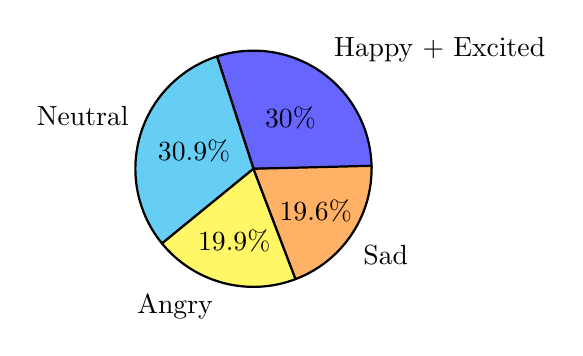
\begin{tikzpicture}
\pie [radius = 1.5]
    {30/Happy + Excited, 30.9/Neutral, 19.9/Angry, 19.6/Sad}
\end{tikzpicture}
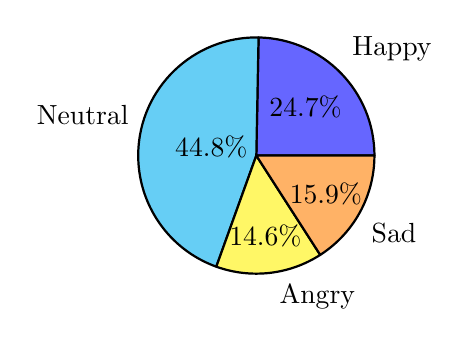
\begin{tikzpicture}
\pie [radius = 1.5]
    {24.7/Happy, 44.8/Neutral, 14.6/Angry, 15.9/Sad}
\end{tikzpicture} \\
Abb. 1: Prozentuale Verteilung der Emotionsklassen in IEMOCAP (links) und MSP-IMPROV (rechts). \\ \\
%1272/Happy, 2313/Neutral, 754/Angry, 819/Sad = 5158
%Angry 1103, Happy+Excited 1636, Neutr 1708, Sad 1084 = 5531
Beim Vergleich der beiden Korpora fiel auf, dass Emotionen teils unterschiedlich gespielt wurden - während wir in IEMOCAP die "traurigen" Sprachproben als leise und in betroffenem Tonfall vorgetragen wahrnahmen, wirkten die Proben der gleichen Klasse in MSP-IMPROV eher aufgelöst und frustriert. \\ \\
Die beiden Datensätze wurden mit zwei unterschiedlichen Machine-Learning-Verfahren benutzt, einem Decision Tree (DT) und einem Support Vector Classifier (SVC). Hierfür wurden die in der Open Source Bibliothek Scikit-learn zur Verfügung gestellten Module SVC und Decision Tree Classifier verwendet. Die Module wurden jeweils von Hand in Python 3 implementiert. 

(Welche Module? Welche Einstellungen?)

\section{Ergebnisse}

\subsection{Versuche}

\subsubsection{Baselinesysteme für DT und SVC auf IEMO (2, 5 zsm) und MSP (ohne P)}

\begin{tabular}{|r|llll|}
\hline
GS / DT & A & H & N & S \\
\hline
A & 194 & 69 & 53 & 11 \\
H & 88 & 219 & 156 & 39 \\
N & 34 & 134 & 307 & 62 \\
S & 11 & 21 & 97 & 165 \\
\hline
\end{tabular}
\begin{tabular}{|r|llll|}
\hline
GS / DT & A & H & N & S \\
\hline
A & 55 & 78 & 82 & 5 \\
H & 31 & 153 & 161 & 13 \\
N & 52 & 105 & 499 & 62 \\
S & 12 & 26 & 136 & 78 \\
\hline
\end{tabular} \\

Abb. 1: Konfusionsmatrix zu IEMOCAP (links) und MSP-IMPROV (rechts) mit Decision Tree, Reihen: Gold Standard, Zeilen: DT. \\ \\
Auffällig sind hier die stark unterschiedlichen Ergebnisse des Decision Trees im Bezug auf die Klassen Angry und Sad: Auf IEMOCAP erreicht Angry mit 0.6 den höchsten F1-Score und Sad den zweithöchsten mit 0.58, auf MSP-IMPROV wird Angry dagegen am schlechtesten erkannt (F1-Score von 0.3) und Sad am zweitschlechtesten (F1-Score 0.38). Für Happy und Neutral werden vergleichbare F1-Scores erreicht (0.54 (IEMOCAP) und 0.42 (MSP-IMPROV) für Happy, 0.54 (IEMOCAP) und 0.63 (der höchste F1-Score auf MSP-IMPROV) für Neutral). 

Der Decision Tree performt auf IEMOCAP im Bezug auf die unterschiedlichen Klassen verhältnismäßig ausgeglichen, während auf MSP-IMPROV größere Unterschiede zwischen den F1-Scores vorliegen. Insgesamt performt der Decision Tree auf IEMOCAP besser. \\ \\ \\
\begin{tabular}{|r|llll|}
\hline
GS / SVC & A & H & N & S \\
\hline
A & 113 & 138 & 47 & 29 \\
H & 33 & 240 & 173 & 56 \\
N & 4 & 124 & 287 & 122 \\
S & 1 & 21 & 68 & 204 \\
\hline
\end{tabular} 
\begin{tabular}{|r|llll|}
\hline
GS / SVC & A & H & N & S \\
\hline
A & 26 & 50 & 144 & 0 \\
H & 13 & 87 & 258 & 0 \\
N & 12 & 47 & 659 & 0 \\
S & 6 & 15 & 230 & 1 \\
\hline
\end{tabular} \\

Abb. 2: Konfusionsmatrix zu IEMOCAP (links) und MSP-IMPROV (rechts) mit Support Vector Classifier, Reihen: Gold Standard, Zeilen: SVC. \\

Der Support Vector Classifier performt auf IEMOCAP für Sad am besten (F1-Score 0.58), auf MSP-IMPROV dagegen am schlechtesten (F1-Score 0.01). Happy und Angry werden sowohl auf IEMOCAP als auch auf MSP-IMPROV nur schlecht erkannt: Auf IEMOCAP erreichen die beiden Klassen mit 0.47 den niedrigsten F1-Score, auf MSP-IMPROV sogar nur 0.31 für Happy und 0.19 für Angry. 
Neutral wird auf beiden Korpora gut erkannt (F1-Score von 0.52 für IEMOCAP, 0.66 für MSP). Auch hier performt der Classifier auf IEMOCAP ausgeglichener über die einzelnen Klassen und insgesamt besser als auf MSP-IMPROV. 

Die großen Unterschiede zwischen den F1-Scores für MSP-IMPROV sind hierbei zum Teil auf die stark unterschiedlichen Klassengrößen im Korpus zurückzuführen (SIEHE KUCHENDIAGRAMM IN METHODEN?)

\subsubsection{Baseline DT und SVC auf Emotionspaaren}

Um die Unterschiede in der Performance unserer Systeme auf den Korpora näher zu untersuchen führen wir Tests auf Emotionspaaren aus. Dabei nutzen wir jeweils nur die Daten aus zwei Emotionsklassen eines Datensatzes als Input, um genau zu erkennen, welche Emotionen besonders gut oder schlecht zu unterscheiden sind. \\ \\
DecisionTree: \\
Zunächst führen wir die Experimente mit dem DT durch.
Dabei lässt sich erkennen, dass das Emotionspaar aus den Klassen Happy und Angry mit beiden Datensätzen schwer zu unterscheiden ist. Bei Training mit Daten aus MSP-IMPROV werden Daten aus A besonders oft als H vorhergesagt.
Das Emotionspaar aus angry und sad wird hingegen mit beiden Datensätzen jeweils sehr gut unterschieden.
Mit Daten aus MSP-IMPROV fällt auf, dass viele Daten aus anderen Emotionsklassen oft fälschlicherweise Neutral zugeordnet werden. Dies lässt sich vermutlich auf Unterschiede in den Datenmengen pro Klasse zurückzuführen, denn die Neutral-Klasse von MSP ist deutlich größer als die anderen. \\
- - Hinweis auf Diagramm zu Klassengrößen? - - \\ \\
SupportVectorClassifier: \\
Wir wiederholen das Experiment mit dem SVC.
Wieder werden die Emotionen happy und angry auf beiden Datensätzen am schlechtesten unterschieden. Mit MSP-IMPROV werden Daten aus Angry noch öfter als Happy vorhergesagt, sodass der recall der Klasse Angry nur 0,15 beträgt.
Vergleiche mit Neutral sind mit dem SVC auf MSP-IMPROV noch schlechter als mit dem DT. Daten aus Happy, Angry und Sad werden meistens als Neutral vorhergesagt, keine der drei Klassen erzielen einen recall über 0,33.
Das Emotionspaar aus Neutral und Sad wird mit Training auf IEMOCAP gut unterschieden, mit Training auf MSP-IMPROV hingegen wird die Klasse Sad überhaupt nicht benutzt. \\ \\
Schlussfolgerung: \\
Auf beiden Systemen sind mit beiden Datensätzen die Klassen Happy und Angry besonders schwer zu unterscheiden. Angry und Sad hingegen werden in allen Versuchen gut unterschieden. Zudem können wir feststellen, dass der Größenunterschied zwischen den Klassen einen großen Einfluss auf die Performance unserer Systeme hat, besonders auf den SVC. \\
- - Mögliche Begründung für Performance von H\&A/ A\&S? - - \\ \\

\subsubsection{DT und SVC auf MSP, alle Klassen gleich groß}

\begin{tabular}{|r|llll|}
\hline
GS / DT & A & H & N & S \\
\hline
A & 134 & 55 & 15 & 21 \\
H & 61 & 120 & 25 & 15 \\
N & 23 & 43 & 130 & 52 \\
S & 37 & 40 & 32 & 102 \\
\hline
\end{tabular}
\begin{tabular}{|r|llll|}
\hline
GS / SVC & A & H & N & S \\
\hline
A & 120 & 56 & 19 & 30 \\
H & 47 & 102 & 29 & 43 \\
N & 10 & 30 & 138 & 70 \\
S & 34 & 31 & 52 & 94 \\
\hline
\end{tabular} \\

Abb. 1: Konfusionsmatrix von DT (links) und SVC (rechts) auf MSP-IMPROV mit angeglichener Klassengröße, Reihen: Gold Standard, Zeilen: DT. \\

Da unsere Ergebnisse zuvor durch die ungleichen Klassengrößen in MSP-IMPROV beeinflusst wurden, wiederholen wir unsere Experimente mit angeglichenen Klassengrößen. Dazu beschränken wir alle Klassen aus MSP auf die Größe der kleinsten Klasse, welche 754 Datenpunkte enthält. \\
Zunächst testen wir beide Systeme auf den beschränkten Klassen. \\ \\
DecisionTree: \\
Alle Klassen werden deutlich besser erkannt, die Performance ist insgesamt ausgeglichener. Vor allem sad und angry werden deutlich besser erkannt.
Neutral performt weiterhin am besten, am schlechtesten werden Sad und Happy erkannt. Mit der Begrenzung performt der DT auf MSP-IMPROV nun genauso gut wie auf IEMOCAP. \\
- - Tabellen/ Matrizen - - \\ \\
SupportVectorClassifier:
Wie beim DT ist die Perfomance deutlich ausgeglichener. Alle Emotionen werden deutlich besser erkannt, wobei Neutral noch immer am besten und sad am schlechtesten erkannt wird. \\
- - Tabellen/ Matrizen - - \\ \\
Schlussfolgerung: \\
Das Angleichen der Klassengrößen hat die Performance deutlich verbessert.
Beim DT hat sich auch das Verhältnis der Performance auf den Klassen geändert, sodass die Klasse Angry, die zuvor am schlechtesten Performt hat, nun besser erkannt wird als Happy und Sad. Obwohl die Performance nun der mit IEMOCAP ähnelt, wird Sad von beiden Systemen, trainiert auf MSP-IMPROV, am schlechtesten erkannt. Dieser Unterschied scheint Korpusabhängig zu sein. \\ \\

\subsubsection{DT und SVC auf MSP mit begrenzten Klassengrößen auf Emotionspaaren}

Nachdem die Begrenzung der Klassengrößen in MSP-IMPROV bei beiden Systemen zu einer deutlichen Verbesserung der Performance geführt hat, führen wir nun wie in 3.1.1 (!!!später Ref Einfügen!!!) Tests auf Emotionspaaren durch. \\ \\
DecisionTree: \\
Das Emotionspaar aus den Klassen Happy und Angry ist noch immer am schwersten zu unterscheiden. Emotionen im Emotionspaar mit Neutral werden nun ebenfalls deutlich besser erkannt. \\
- - Konfusionsmatrix - - \\ \\
SupportVectorClassifier: \\
Wie zuvor wird auch mit dem SVC das Emotionspaar aus Happy und Angry noch immer am schlechtesten unterschieden. Auch hier wird in Emotionspaaren, die Neutral enthalten, nun deutlich besser zwischen den beiden Emotionen unterschieden. Im Emotionspaar aus Sad und Neutral werden beide Klassen nun gleich gut erkannt. \\
- - Konfusionsmatrix - - \\ \\
Schlussfolgerung: \\
Auch in den Emotionspaaren hat das Anpassen der Klassengrößen die Performance deutlich verbessert. Das Emotionen happy und angry werden noch immer am schlechtesten unterschieden. \\

\subsubsection{Decision Tree auf Kombinationen von IEMO und MSP}
\begin{tabular}{|r|llll|}
\hline
GS / DT & A & H & N & S \\
\hline
A & 241 & 467 & 35 & 3 \\
H & 330 & 836 & 92 & 3 \\
N & 537 & 1429 & 307 & 20 \\
S & 112 & 534 & 137 & 24 \\
\hline
\end{tabular}
\begin{tabular}{|r|llll|}
\hline
GS / DT & A & H & N & S \\
\hline
A & 178 & 411 & 278 & 224 \\
H & 106 & 466 & 607 & 444 \\
N & 100 & 228 & 656 & 706 \\
S & 69 & 54 & 320 & 629 \\
\hline
\end{tabular} \\
\begin{tabular}{|r|llll|}
\hline
GS / DT & A & H & N & S \\
\hline
A & 254 & 133 & 138 & 25 \\
H & 180 & 317 & 312 & 76 \\
N & 104 & 214 & 722 & 161 \\
S & 22 & 56 & 250 & 243 \\
\hline
\end{tabular} \\

Abb. 1: Konfusionsmatrix zu DT, links trainiert auf IEMOCAP und getestet auf MSP-IMPROV, rechts trainiert auf MSP-IMPROV und getestet auf IEMOCAP, unten trainiert und getestet auf Kombination beider Korpora, Reihen: Gold Standard, Zeilen: SVC. \\
Der auf IEMOCAP trainierte Decision Tree performt auf MSP-IMPROV (unbegrenzt) am besten für Happy (Höchster F1-Score mit 0.37, höchster Recall mit 0.66, allerdings niedrige Precision mit 0.26). Angry erreicht einen Recall von 0.32 und mit 0.2 die schlechteste Precision. Neutral und Sad erreichen mit 0.13 und 0.03 die schlechtesten Werte für Recall und mit 0.21 und 0.06 die schlechtesten Werte für den F1-Score, erzielen aber mit 0.54 und 0.48 die höchste Precision. 
Insgesamt werden die Daten anderer Klassen nun meist als Happy klassifiziert. Daten aus Happy werden oft unter Angry eingeordnet. 

Trainiert man den DT auf MSP-IMPROV und testet ihn dann auf IEMOCAP, erreicht Sad mit 0.59 den höchsten Recall und trotz der niedrigsten Precision (0.31) mit 0.41 den höchsten F1-Score. 
Happy und Angry erreichen hier mit 0.4 und 0.39 die höchste Precision, aber mit 0.29 und 0.16 den niedrigsten Recall. F1-Scores sind 0.34 für Happy und 0.23 für Angry. Neutral wird mit Precision 0.35, Recall 0.39 und F1-Score 0.37 verhältnismäßig gut erkannt. 
Der DT verwechselt oft Sad und Neutral miteinander. Angry wird vor allem Happy zugeordnet. Happy wird hauptsächlich als Neutral erkannt. 

Trainiert und testet man den DT auf einer Kombination beider Korpora, wird Neutral mit einem F1-Score von 0.55, einem Recall von 0.6 und einer Precision von 0.51 am besten erkannt. Happy wird am schlechtesten erkannt (Precision 0.44, Recall 0.36, F1-Score 0.4) und oft Neutral zugeordnet. Sad (Precision 0.48, Recall 0.43, F1-Score 0.45) und Angry (Precision 0.45, Recall 0.46, F1-Score 0.46) werden verhältnismäßig gut erkannt, wobei Sad häufiger Neutral zugeordnet wird als sich selbst und Angry häufig Neutral und Happy. 

\subsubsection{Support Vector Classifier auf Kombinationen von IEMO und MSP}

SVC_Kombination_IEMO_MSP \\
\begin{tabular}{|r|llll|}
\hline
GS / SVC & A & H & N & S \\
\hline
A & 495 & 203 & 42 & 6 \\
H & 684 & 419 & 156 & 2 \\
N & 787 & 783 & 700 & 23 \\
S & 186 & 402 & 206 & 13 \\
\hline
\end{tabular}
\begin{tabular}{|r|llll|}
\hline
GS / SVC & A & H & N & S \\
\hline
A & 1 & 313 & 777 & 0 \\
H & 2 & 243 & 1376 & 2 \\
N & 2 & 69 & 1618 & 1 \\
S & 0 & 49 & 1021 & 2 \\
\hline
\end{tabular} \\
\begin{tabular}{|r|llll|}
\hline
GS / SVC & A & H & N & S \\
\hline
A & 99 & 226 & 211 & 14 \\
H & 65 & 321 & 460 & 39 \\
N & 23 & 179 & 918 & 81 \\
S & 8 & 40 & 383 & 140 \\
\hline
\end{tabular} \\

Abb. 1: Konfusionsmatrix zu SVC, links trainiert auf IEMOCAP und getestet auf MSP-IMPROV, rechts trainiert auf MSP-IMPROV und getestet auf IEMOCAP, unten trainiert und getestet auf Kombination beider Korpora, Reihen: Gold Standard, Zeilen: SVC. \\

Testet man den auf IEMOCAP trainierten SVC auf MSP-IMPROV, wird Sad sehr schlecht erkannt (Recall 0.02)und hauptsächlich Happy zugeordnet. Neutral wird ca. zu je einem Drittel Angry, Happy und sich selbst zugeordnet (Recall 0.31). Happy (Recall 0.33) wird häufiger Angry zugeordnet als sich selbst. Angry wird gut erkannt (Recall 0.66) und teils Happy zugeordnet. 

Testet man den auf MSP-IMPROV trainierten SVC auf IEMOCAP, werden Angry und Sad fast gar nicht verwendet (Precision je 0.2 und 0.4, Recall und F1-Score jedoch für beide 0). Happy wird fast vollständig Neutral zugeordnet (Recall von 0.15). Neutral wird mit einem Recall von 0.96 sehr gut erkannt (F1-Score 0.5). 

Trainiert und testet man den SVC auf beiden Korpora, wird Neutral mit einem Recall von 0.76 (F1-Score 0.58) am besten erkannt. Angry wird mit einem Recall von 0.18 (F1-Score 0.27) am schlechtesten erkannt und meist Happy oder Neutral zugeordnet. Sad wird ebenfalls nur schlecht erkannt (Recall 0.25, F1-Score 0.33) und meist Neutral zugeordnet. Happy wird häufiger richtig eingeordnet (Recall 0.36, F1-Score 0.39), aber ebenfalls meist Neutral zugeordnet. 

\subsection{notes}

Vergleich IEMOCAP / MSP-IMPROV
Wenn man das Modell auf den einen Korpus trainiert und mit dem anderen testet, verschlechtert sich die performance extrem, z. B. bei sad. Auffällig: Emotionen werden in den Korpora anders geschauspielert, in IEMOCAP ist Sad zum Beispiel sehr ruhig, in MSP-IMPROV sind die Personen auf sehr aufgebrachte Art traurig/aufgelöst
-> Wie definiert man, wie Emotionen klingen sollen?

Wenn man auf MSP-IMPROV trainiert und auf IEMOCAP testet, wird Sad in Neutral geschoben (weil Sad in IEMOCAP nicht so extrem aufgelöst klingt?

\subsection{Diskussion}

Wenn man auf MSP-IMPROV trainiert und auf IEMOCAP testet, wird Sad in Neutral geschoben (weil Sad in IEMOCAP nicht so extrem aufgelöst klingt?

Angry ist aber zum Beispiel gut zu erkennen, obwohl die Klasse kleiner als Sad ist, vielleicht weil Angry einen sehr charakteristischen Klang hat?

SVC hat Probleme wenn Klassen im Umfang stark schwanken (= in manchen hunderte von samples sind und in manchen nur ein 5 oder 6) (was bei MSV_IMPROV so war was vermutlich ein Faktor ist warum die VSC hier schlechter performt)
SVC performt auf IEMOCAP auch schlechter seit wir Happy und Excited kombiniert haben(?)

\section{Zusammenfassung}

Schwierigkeit: Wie definiert man, wie Emotionen klingen sollen? Soll z.B. sad laut und aufgelöst sein oder ruhig und zurückgezogen? (Oft auch kulturelle Unterschiede?)

Verbesserungsvorschläge und so: Wir hätten Korpora nachbearbeiten können (z. B. stille Teile von MSP-IMPROV abschneiden)

Etwa gleichgroße Klassengröße verbessert performance auf jeden Fall

Neutral wird gut erkannt weil größte Klasse, andere Emotionen werden N aus diesem Grund sehr oft falsch zugeordnet, aber es ist halt auch neutral

bestimmte Emotionen werden besonders gut oder schlecht erkannt, auch Korpus abh.

\pagebreak
\tableofcontents
\pagebreak
\bibliography{iclr2020_conference}
\bibliographystyle{iclr2020_conference}

\end{document}
